\documentclass{article}

\usepackage[final]{neurips_2018}

\usepackage[utf8]{inputenc} % allow utf-8 input
\usepackage[T1]{fontenc}    % use 8-bit T1 fonts
\usepackage{hyperref}       % hyperlinks
\usepackage{url}            % simple URL typesetting
\usepackage{booktabs}       % professional-quality tables
\usepackage{amsfonts}       % blackboard math symbols
\usepackage{nicefrac}       % compact symbols for 1/2, etc.
\usepackage{microtype}      % microtypography

\usepackage{graphicx}
\usepackage{wrapfig}
\usepackage{amsmath}
\usepackage{amssymb}
\usepackage{lipsum}

\newcommand{\Nn}{\mathbf{N}}
\newcommand{\Rr}{\mathbf{R}}
\newcommand{\Pp}{\mathbb{P}}
\newcommand{\Ee}{\mathbb{E}}

\title{Hierarchical reinforcement learning}

\author{%
  Guillaume DALLE \\
  École Nationale des Ponts et Chaussées \\
  \texttt{guillaume.dalle@eleves.enpc.fr} 
  \And
  Clément MANTOUX \\
  École polytechnique \\
  \texttt{clement.mantoux@polytechnique.edu}
}

\begin{document}
% \nipsfinalcopy is no longer used

\maketitle

\begin{abstract}

Hierarchical Reinforcement Learning attempts to solve complex, multiscale problems by breaking them down into smaller subtasks. This decomposition, either provided by an expert or devised automatically, is often necessary to make the learning process faster, or indeed feasible at all. We review different approaches to hierarchical modelling and structure detection in reinforcement learning, with an emphasis on the role of the framework.

\end{abstract}

\section{Introduction}  \label{intro}

\subsection{Problem statement}

Reinforcement learning (RL) deals with problems in which an agent interacts with a (sometimes unknown) environment, and tries to maximize their reward by designing an optimal policy. While standard optimization methods such based on dynamic programming work well in many small-scale situations, learning to perform complex tasks, from robot control to autonomous driving, is still a major challenge.

The reason is that such endeavours are hard to represent using only primitive, atomic actions lasting one time-step. It is better to divide the problem into macroscopic (multi-step) subtasks first, then possibly divide these subtasks into smaller ones, etc.  This multiscale decomposition goes on until reaching the level of primitive actions. Then, the increasingly abstract subtasks can be reconstructed and learned from the bottom up, enabling the agent to solve the initial problem. 
Hierarchical Reinforcement Learning (HRL) aims to integrate this hierarchical decomposition idea into standard RL algorithms. This is meant to speed up the learning process by restricting the search space or giving the learning algorithm more powerful exploration abilities. We will try to give a brief overview of this recent field, with two fundamental questions in mind:
\begin{itemize}
    \item How can one represent and use a given hierarchy of subtasks?
    \item How can one automatically learn the right hierarchical structure for a given problem? 
\end{itemize}

The rest of section \ref{intro} introduces the mathematical framework underlying most RL algorithms. In section \ref{representing}, we present and compare several different ways to express a known hierarchical decomposition. Then, in section \ref{learning}, we tackle the issue of learning an appropriate structure of subtasks, listing both classical and deep learning technniques.

\subsection{(Semi-)Markov Decision Processes and Reinforcement Learning}

Most of the literature on Reinforcement Learning uses the Markov Decision Process (MDP) setting. An MDP is a mathematical model describing the interactions between an agent and an environment. At each discrete time step $t \in \Nn$, the agent finds itself in a state $s_t \in S$, where it can choose an action $a_t \in A$. This action triggers a transition to state $s_{t+1}$ according to conditional probabilities $p(s_{t+1} | s_t, a_t)$, and the agent receives a random reward $r_t$ whose expectation is $r(s_t, a_t)$.

A deterministic policy $\pi: S \to A$ can be evaluated either with the state value function $V^{\pi}: S \to \Rr$, which computes the expected discounted reward when following policy $\pi$ from a given state, or with the state-action value function $Q^{\pi}: S \times A \to \Rr$. The agent's goal is to find an optimal policy, ie. a policy $\pi^*$ reaching the maximum possible value $V^*(s) = \max_{\pi} V^{\pi}(s)$ in each state $s$. Both the value functions and the optimal value functions satisfy Bellman equations similar to:
\begin{equation}
    Q^* (s, a) = r(s, a) + \gamma \sum_{s'}{p(s' | s, a) \max_{a'}{Q(s', a')}}
\end{equation}
Bellman equations form the basis of RL algorithms such as Q-learning \cite{watkins_q-learning_1992}, which allow the agent to learn the transitions and rewards associated with an unknown environment.

Semi-Markov Decision Processes (SMDP) have the same ground rules, except that the actions can last for $\tau > 1$ time steps, leading to duration-dependent transition probabilities $p(s', \tau | s, a)$. They are the adequate tool to represent situations where the agent may perform multi-step combinations of actions in order to achieve a subtask.

\section{Representing the hierarchy} \label{representing}

The basic situation in Hierarchical Reinforcement Learning is the one in which the hierarchy of subtasks is given, most of the time thanks to expert knowledge of the problem at hand. Along the lines of \cite{barto_recent_2003}, we introduce four different proposals to translate the hierarchical structure into a learnable model. We then discuss and compare these approaches.

These proposals will all be illustrated using always the same kind of toy problem inspired by both \cite{dietterich_hierarchical_2000} and \cite{sutton_between_1999}. It consists of a navigation challenge in a room-like grid world (see figure \ref{fig:svi}), where the agent must go from a source cell to a target cell, possibly picking up and dropping off a passenger along the way.

\subsection{Feudal Reinforcement Learning (FRL)}

The first approach we discuss was introduced by Dayan and Hinton \cite{dayan_feudal_1993} and embraces a medieval analogy for absolute hierarchical control. The levels $\ell$ of the hierarchy correspond to partitions $\mathcal{P}_{\ell} = \{R_{\ell, j}, j \in [n_{\ell}]\}$ of the state space into increasingly large regions, each supervised by a manager $m_{\ell, j}$. The bottom level $\ell = 0$ corresponds to the granularity at which the agent can act, and the others correspond to increasing levels of abstraction. At every time step, every active manager $m_{\ell, j}$ (supervising a region containing the agent's state $s$):
\begin{itemize}
    \item receives an order $o_{\ell}^+$ from its super-manager $m_{\ell+1, k}$ (st. $R_{\ell+1, k}  \supset R_{\ell, j}$)
    \item gives an order $o_{\ell}^-$ to its one active sub-manager $m_{\ell-1, i}$ (st. $s \in R_{\ell-1, i} \subset R_{\ell, j}$)
\end{itemize}

In our example, there could be a global manager, then one submanager for each room, and then entry-level managers for each cell. On each level, several orders are available: \texttt{GoNorth}, \texttt{GoSouth}, \texttt{GoEast}, \texttt{GoWest} (orders or actions at level $\ell=0$), and \texttt{FindTarget}, \texttt{GoToRoom($R$)} (abstract orders, available only in the upper levels). The order given by a manager is encoded into the state of its sub-manager, but the sub-manager doesn't understand what the order means at first. Hence the manager also has to set the rewards for his sub-manager, so that it learns which of his actions is best to execute a given order.

The global task by each manager simultaneously applying a Q-learning scheme on its own Q-function $Q[(s, o_{\ell}^+), o_{\ell}^-]$, which it approximates through the rewards decided from above, and which it uses to determine what order will be sent downwards.

\subsection{Hierarchies of Abstract Machines (HAM)}

The second approach we describe is due to Parr and Russel \cite{parr_reinforcement_1998} and draws from the theory of finite automata. Indeed, we add to the MDP a layer of \emph{machines} designed to control it by performing specific subtasks. A machine is defined by a set of states linked by a transition function. There are four machine states: \texttt{Action} (executes an action in the original MDP), \texttt{Call} (calls another machine), \texttt{Choice} (selects a next machine state with given probabilities) and \texttt{Stop} (terminates the execution and goes back to the last call).

\begin{wrapfigure}{r}{5cm}
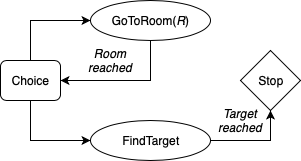
\includegraphics[width=5cm]{images/HAM.png}
\caption{An example of machine in charge of navigation}
\label{fig:HAM}
\end{wrapfigure}

For instance, in our room navigation challenge, there could be a machine (depicted in figure \ref{fig:HAM}) dedicated to navigating towards a given target. It would have two possible calls: either check the current room for the target or go to another one, both being implemented by other sub-machines (which can make use of primitive actions).

If we denote by $H$ the set of machines and by $M$ the original MDP, then the resulting object $H \circ M$ is an SMDP. Its states are pairs of states of $H$ and $M$, and its actions are the possible next states at each machine \texttt{Choice}. After such a decision, the system runs autonomously for several time steps, until another \texttt{Choice} is reached. With a suitable reduction (considering only pairs of states with a \texttt{Choice} component),  $H \circ M$ becomes much less complex than $M$, and can thus be learned quickly with standard MDP algorithms. More details on the learning algorithm (called HAMQ) are given in Parr's PhD dissertation \cite{parr_hierarchical_1998}. 

\subsection{MAXQ decomposition}

\begin{wrapfigure}{l}{7cm}
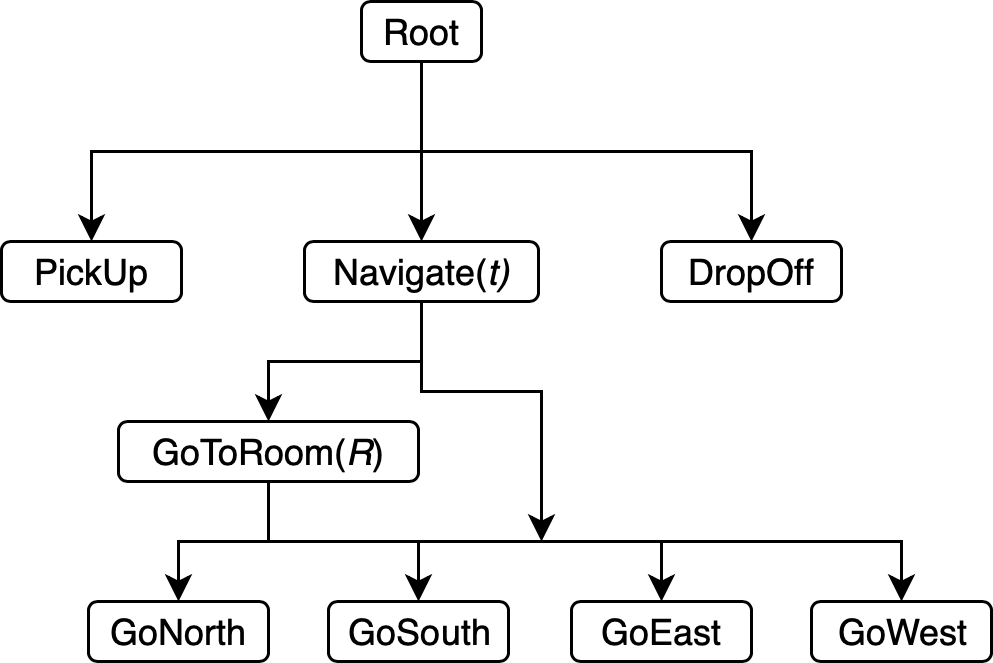
\includegraphics[width=7cm]{images/MAXQ.png}
\caption{Task graph for the MAXQ decomposition}
\label{fig:MAXQ}
\end{wrapfigure}

The third approach we present was imagined by Dietterich \cite{dietterich_hierarchical_2000}, and it is based on a subtask graph. Let us go back to the illustrating example of navigating between rooms, with the added mission of picking up and dropping off an object along the way. Then the subtask graph could look like the one in figure \ref{fig:MAXQ}. The root task is our main challenge, and each child of a node represent a possible subtask this node can use to perform its own mission. The leaves of the graph are primitive actions.

Formally, this is expressed by decomposing the original MDP $M$ into a set of subtasks $M_i$, each being composed of three components: $T_i$ (a termination predicate indicating states where $M_i$ is over), 
$A_i$ (the set of actions or subtasks available to achieve $M_i$) and
$\tilde{R}_i(s)$ (a local pseudo-reward function for terminal states of $M_i$). Given this hierarchical decomposition, a hierarchical policy $\pi$ is a set of policies $\pi_i$ for each subtask, such that $\pi_i$ only uses elements of $A_i$. To apply such a policy, it is necessary to use a stack-based algorithm to keep track of all the subtasks currently executing.

Let us define the projected value function $V^{\pi}(s, a)$ as the expected cumulative reward of executing $\pi_a$ from state $s$ until subtask $M_a$ is over. A key observation is that each subtask $M_i$ where the hierarchical policy $\pi$ is applied defines a SMDP. In this SMDP, the expected reward $r(s, a)$ of each action $a \in A_i$ is equal to its projected value function $V^{\pi}(a, s)$. Furthermore, the Bellman equations here are decomposition equations:
\begin{equation}
    Q^{\pi}(i, s, a) = V^{\pi}(s, a) + C^{\pi}(i, s, a) \quad \text{and} \quad V^{\pi}(s, i) = \begin{cases} Q^{\pi}(i, s, \pi_i(s)) & \text{composite $i$} \\ r(s, i) & \text{primitive $i$} \end{cases}
\end{equation}

In other words, the reward induced by policy $\pi$ on subtask $i$, if it starts on state $s$ with action $a$, can be decomposed into the projected value of state $s$ in subtask $a$ plus a certain completion function.
Therefore, all that is needed to reconstruct the value function are the quantities $[V^{\pi}(a, s)]_s$ for all primitive actions $a$ and $[C^{\pi}(i, s, a)]_{s, a}$ for all composite subtasks $i$. This is at the heart of the recursive MAXQ-0 algorithm, which learns a recursively optimal policy by iteratively updating the $V^{\pi}$ and $C^{\pi}$ values in a stochastic approximation scheme. The MAXQ-Q extension deals with the general case of non-zero pseudo-rewards $\tilde{R}$, which can speed up learning by directing the search.

\subsection{Options}

The fourth approach we detail is the options framework, which was introduced by Sutton, Precup and Singh \cite{sutton_between_1999} and is the basis of much of the modern research on HRL. It forms an extension of the classical MDP setting, where we consider sequences of actions with extended time durations, the so-called \textit{options}.

Formally, we define an option $\omega \in \Omega$ as a tripel $(\mathcal{I}_\omega, \pi_\omega, \beta_\omega)$. The initiation set $\mathcal{I}_\omega \subset \mathcal{S}$ is the set of states where the option is available. Once an option is selected, the agent follows the non-deterministic policy $\pi_\omega$, until the option stochastically terminates with probability $\beta_\omega$ depending on the current state. Primitive actions are then special cases of options that always terminate after one step. Note that the policies $\pi_\omega$ can  depend on the history of states, actions and rewards since the initiation of the option (and not only on the current state $s_t$), which makes it "semi-Markov".

With these notations, an episode unfolds as follows: the agent picks an option to start with, and follows its policy until it terminates, then it chooses another option, and so on until termination. The options are chosen with a \textit{policy over options} $\pi_\Omega : \mathcal{S} \times \Omega \rightarrow [0, 1]$. An MDP endowed with an options set $\Omega$ and a policy $\pi_\Omega$ is thus an SMDP : the actions of the SMDP are the options in the MDP.
The value functions easily generalize: for instance we can define the option-value function $Q^{\pi_\Omega} : \mathcal{S} \times \Omega \rightarrow \Rr$ and the optimal option-value function $Q^*_\Omega$ as follows :
\begin{equation}
\begin{cases}
Q^{\pi_\Omega}(s, \omega) = \Ee[r_1 + \gamma r_2 + \gamma^2 r_3 +  ... \mid s_0 = s, \omega_0 = \omega] \\
Q^*_\Omega(s, \omega) = \max_{\pi_\Omega} Q^{\pi_\Omega}(s, \omega)
\end{cases}
\end{equation}

\begin{wrapfigure}{r}{7cm}
    \centering
    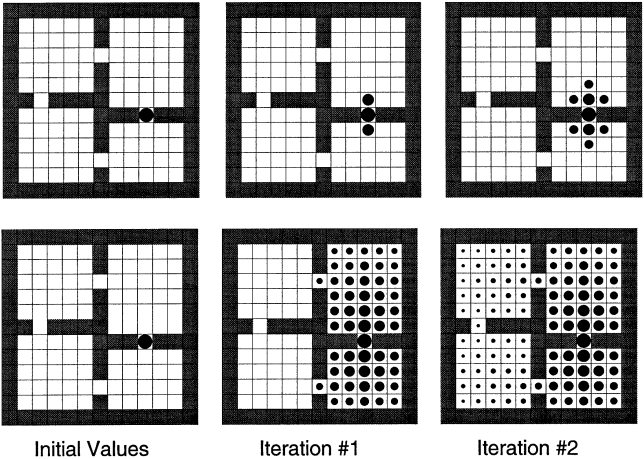
\includegraphics[width=7cm]{images/SVI_options.png}
    \caption{Synchronized Value Iteration with options. \small \it The grids display the value of each state at each iteration. The first row shows the classical MDP value iteration, and the second row shows the same result with hallway-reaching options. The value propagates much faster in the second setting.}
    \label{fig:svi}
\end{wrapfigure}

These values are suboptimal compared with the MDP's classical value functions since the primitive actions may not be available as options : this is the price of the abstraction. Yet, these functions satisfy generalized Bellman equations which can be used to derive learning algorithms.

In the original article \cite{sutton_between_1999}, the options structure is given. In this situation, the authors show that well selected options drastically speed up the convergence of estimation algorithms. In figure \ref{fig:svi}, we show their experiment in the four rooms problem. The Synchronized Value Iteration converges much faster in the MDP with options than in the classical setting.

\subsection{Comparison of the frameworks}

We now discuss the merits and drawbacks of the four frameworks introduced above, by comparing them along several axes.

\paragraph{Information to supply}

Goals vs policies, local rewards

\paragraph{Mathematical complexity}

\paragraph{Convergence} Hierarchically optimal / recursively optimal for MAXQ

\paragraph{Recursive depth} 2 for options, more for the reste

\paragraph{Interruption}

\paragraph{State abstraction}

Multiple similar tasks must be learned separately

\section{Learning the hierarchy} \label{learning}

Now that we have several methods to represent a given hierarchy of subtasks, we have to ask how to learn one automatically. We will present a few approaches in detail, spread across multiple frameworks and covering both classical and deep learning techniques.

\subsection{Classical approaches}

\subsubsection{Bottleneck states for option discovery}

Sutton et al.'s options formulation \cite{sutton_between_1999} is by far the most widely used when trying to learn the hierarchical structure of a task, because it lends itself naturally to the definition of subgoals. Note that simply finding a subgoal is not enough: the local policy allowing to reach it must also be computed. This is often done separately in the articles listed below.

The first idea to define relevant subgoals in an MDP is to look for milestone states, ie. states that are critical to the success of a trajectory or the transition between different parts of the state space. , which is the most widely used, 

\begin{itemize}
    \item Multiple instance learning and diverse density \cite{mcgovern_automatic_2001} or relative novelty  \cite{simsek_using_2004}
    \item Generate a graph representing the MDP's exploration history, and apply min cut \cite{goos_q-cutdynamic_2002} or clustering \cite{mannor_dynamic_2004} or local cut \cite{simsek_identifying_2005}
\end{itemize}

\subsubsection{Recursive hierarchy building for MAXQ-like decompositions}

To find a decomposition adapted to the MAXQ framework (or with some contorsions to the HAM formulation), we have to work a bit more. Indeed, options designed at reaching subgoals simply have to be ordered one after the other, whereas MAXQ subtasks form a directed graph with several levels of abstraction. 

\begin{itemize}
    \item \cite{hengst_discovering_2002} works on factored MDPs by defining subtasks to move between regions where one factor variable is constant.
    \item \cite{jonsson_causal_2006} and \cite{mehta_automatic_2008} are more advanced and use Bayesian networks to model relations between factor variables and actions (worth citing ?)
\end{itemize}

\subsubsection{Intrinsic motivation}

Proposed by \cite{chentanez_intrinsically_2005}.

\subsection{Deep learning approaches}

\begin{itemize}
    \item options (predefined subgoals) + DQN \cite{kulkarni_hierarchical_2016}
    \item option-critic \cite{bacon_option-critic_2016} $\rightarrow$ option discovery
    \item STRAW \cite{alexander_strategic_2016}
    \item Stochastic Deep Networks \cite{florensa_stochastic_2017}
    \item FuN \cite{vezhnevets_feudal_2017} (\& FuDRL \cite{casanueva_feudal_2018} ?)
\end{itemize}

In the wake of the paper by Mnih \textit{et al.} \cite{mnih_human-level_2015} on deep Q-networks (DQN), novel algorithms (\cite{kulkarni_hierarchical_2016, bacon_option-critic_2016, alexander_strategic_2016, casanueva_feudal_2018, florensa_stochastic_2017}) were published over the last few years. Some approaches adapt the classical HRL frameworks into trainable deep learning models. Others take stock on the intrisic abilities of neural networks to build internal representations adapted to the problem structure.

\subsubsection{Deep option-critic}

In \cite{bacon_option-critic_2016}, Bacon \textit{et al.} extended the classical actor-critic method to the options framework.

\subsubsection{Feudal networks}



\small
\bibliographystyle{plain}
\bibliography{HRL}

\end{document}